\documentclass[../main.tex]{subfiles}

\begin{document}

\section{Downloading and Installing Texmaker}
% This is its OWN top-level \section — since it's subfiled
% directly into main.tex (not through the Git bundle), it
% will become Section 2, right after "Git and GitHub Setup".

\subsection{What is Texmaker?}
Texmaker is a free, cross-platform editor for writing and
compiling \LaTeX{} documents. It includes a built-in PDF viewer,
syntax highlighting, and one-click compilation, making it a
popular choice for beginners.

\subsection{Download the Installer}
\begin{enumerate}[leftmargin=*]
    \item Open a web browser and go to
    \url{https://www.xm1math.net/texmaker/download.html}.
    \item Choose the installer matching your operating system
    (Windows, macOS, or Linux).
    \item Click the corresponding download link and save the
    file.
\end{enumerate}

\subsection{Run the Texmaker Installer}
\begin{enumerate}[leftmargin=*]
    \item Locate the downloaded installer file and double-click
    it.
    \item If prompted by your operating system for permission to
    make changes, allow it.
    \item Follow the on-screen prompts, keeping the default
    options, and click \textbf{Install} (or \textbf{Next}) until
    the installation completes.
    \item Click \textbf{Finish}.
\end{enumerate}

\subsection{Open Texmaker}
\begin{enumerate}[leftmargin=*]
    \item \textbf{Windows}: click the \textbf{Start} menu, search
    for ``Texmaker'', and open the application.
    \item \textbf{macOS}: open \textbf{Launchpad} or
    \textbf{Applications} and click \textbf{Texmaker}.
    \item \textbf{Linux}: search for ``Texmaker'' in your
    application menu, or launch it from a terminal:
\end{enumerate}

\begin{lstlisting}
texmaker
\end{lstlisting}

\subsection{Verify the Installation}
\begin{enumerate}[leftmargin=*]
    \item In Texmaker, create a new document
    (\textbf{File} $\rightarrow$ \textbf{New}).
    \item Type a simple test document:
\end{enumerate}

\begin{lstlisting}
\documentclass{article}
\begin{document}
Hello, world!
\end{document}
\end{lstlisting}

\begin{enumerate}[leftmargin=*]
    \item Save the file with a \texttt{.tex} extension.
    \item Click the \textbf{QuickBuild} button (or press F1) to
    compile it.
    
	\begin{center}
    	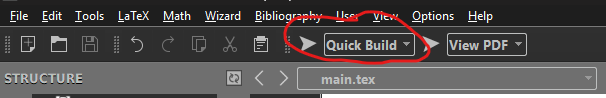
\includegraphics[width=0.7\textwidth]{./Images/QuickBuild.png}
	\end{center}
	
\end{enumerate}

If a PDF preview opens showing ``Hello, world!'', Texmaker and
your \LaTeX{} distribution are installed correctly.

\end{document}